\chapter{CHARACTERISTICS OF A MOBILE DEVICE} \label{cha:character}\index{characteristics}
Compared to the biometric design is this a part of \textit{Choose biometric characteristics}\\
\\
In the hardware of a device there are some features that can be used to distinguish devices from each other. In most cases it is not called features rather error sources, noise or bias. In the aim of this thesis it is feature characteristics that can be seen as an uniqueness of an mobile device. \textit{Device fingerprint(ing)}\index{device fingerprint} is the term used for this feature characteristics and the pyramid seen in~\figureref{fig:pyramid} from ~\cite[]{sensor:acoustic} shows the different types of sources of device fingerprint. This thesis will focus on the top of quarter of that pyramid, that is the sensors. All error sources of sensors comes in form of bias and the bias from each sensor covered by the thesis is further explained in this chapter. There is also an explanation on how the sensors is measured in JavaScript that is used for measurements described in ~\chapterref{cha:measurements}. \\


\begin{figure}[!h]
		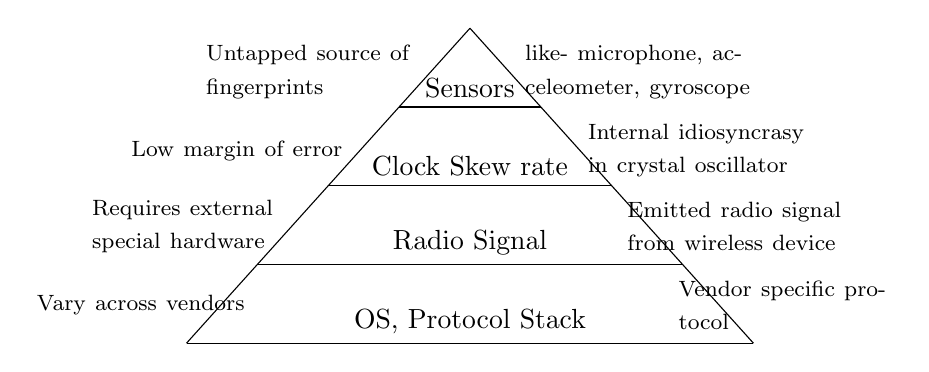
\begin{tikzpicture}[scale=1]

		\def \h {4};
		\def \f {0.9};

		\foreach \y in  {0,1,2,3} {
		    \def \w { \h*\f-\y*\f };
		    \def \v { \y*\f-\h*\f };
		    \draw (\v,\y) -- (\w,\y);
		}

		\draw (-\h*\f,0)  -- (0,\h);
		\draw (\h*\f,0)  -- (0,\h);
		\node (os) at (0,0) [above] {OS, Protocol Stack};
		\node (rf) at (0,1) [above] {Radio Signal};
		\node (cs) at (0,2) [above] {Clock Skew rate};
		\node (se) at (0,3) [above] {Sensors};


		\node [left of=os, xshift=-3cm, yshift=0.2cm, text width=3cm] {\footnotesize{Vary across vendors}};
		\node [left of=rf, xshift=-2.4cm, yshift=0.2cm, text width=2.8cm] {\footnotesize{Requires external special hardware}};
		\node [left of=cs, xshift=-1.8cm, yshift=0.2cm, text width=3cm] {\footnotesize{Low margin of error}};
		\node [left of=se, xshift=-1cm, yshift=0.2cm, text width=2.7cm] {\footnotesize{Untapped source of fingerprints}};

		\node [right of=os, xshift=3cm, yshift=0.2cm, text width=2.7cm] {\footnotesize{Vendor specific protocol}};
		\node [right of=rf, xshift=2.5cm, yshift=0.2cm, text width=3cm] {\footnotesize{Emitted radio signal from wireless device}};
		\node [right of=cs, xshift=2cm, yshift=0.2cm, text width=3cm] {\footnotesize{Internal idiosyncrasy in crystal oscillator}};
		\node [right of=se, xshift=1.2cm, yshift=0.2cm, text width=3cm] {\footnotesize{like- microphone, acceleometer, gyroscope}};
	\end{tikzpicture}
	\caption{\label{fig:pyramid} The pyramid of features in a mobile device that can be used for fingerprinting.\cite[]{sensor:acoustic}}
\end{figure}

As seen above in~\figureref{fig:pyramid} are sensors an untapped source of fingerprints in mobile devices and example of sensors are microphone, accelerometer, barometer, speakers and gyroscope. The sensors investigated in this work is the accelerometer-, gyroscope-, and camera- sensors. All of them are common sensors in most of the mobile devices used today.


\section{Accelerometer\index{accelerometer}}\label{sec:accelerometer}
The accelerometer is the sensor that detect movement on a mobile device, like when you changing orientation on your device. Acceleration is measured by sensing how much pressure the device has in terms of force. The type of accelerometer sensor found in a mobile device is a micro-electromechanical systems known as MEMS sensor. \cite[]{sensors:fusion}
\subsection{Fingerprinting feature / Bias}
Measure the characteristics from the accelerometer is done by taking the long term average of the output when the accelerometer is in rest. That is the biggest error source in the accelerometer and it grows quadratically over time, but when the accelerometer is in rest the error $\epsilon$ can be calculated as a function of time $t$;
\begin{equation} \label{eq:AccBias}
s(t)=\epsilon * \frac{t^2}{2} 
\end{equation}
\cite[]{sensor:inertialNav}\cite[]{sensors:fusion}


\section{Gyroscope\index{gyroscope}}\label{sec:gyroscope}
The gyroscope is sensing how the device is moving in terms of angles, for maintaining or measure the orientation. This is originally  a mechanical system based on the principle of conservation of angular momentum. The most popular Gyroscope for devices today is a MEMS that is using silicon micro-mechanical techniques. Coriolis effect is measured with vibrating elements in the MEMS gyroscope. Coriolis effect is a change of moving objects direction when looking at it from a rotating reference system. The difference from the accelerometer is that the gyroscope measures relative to the device body rather than relative to earth. The equations of Coriolis force;  
$$\boldsymbol{ F}_C = -2 \, m \, (\omega *  v)$$
Where $m$ is the mass of the particle, $\omega$ the angular velocity and $v$ the velocity of the particle in the rotating system. 
\cite[]{sensor:inertialNav}
\subsection{Fingerprinting feature / Bias}
The gyroscope has some error characteristics like constant bias, white noise, bias instability, calibration error and temperature effects. One of these error characteristics that can be tested by reading the output from a gyroscope in rest is the \textit{constant bias}\index{constant bias}. That is bias of the gyroscope output when not having any rotation on it. This constant error $\epsilon$ of the bias over time $t$ leads to an angular error that grows linear; 
\begin{equation} \label{eq:gyroBias}
\theta (t)= \epsilon * t
\end{equation}
If take the long term average output from the gyro in rest, the constant error of a rate gyro can be estimated.\cite[]{sensors:fusion}


\section{Camera}\label{sec:char:camera}\index{camera fingerprinting}\index{camera}
\textit{Note that normally bias in a camera sensor is called \textbf{noise} but for uniformity reason of this report it will be referenced to \textbf{bias}.}\\
\\
The digital camera of a mobile device also includes sensors and other hardware that can be used as fingerprinting characteristics. The basic is that light travels trough a lens and hits a imaging sensor which contains pixels that has a filter array in front. The filter is for gives each pixel a detected color. The pixels is then put together again to a resulting signal which is send to some final post processing (color correction, white balance, etc.) steps before the image is written to the memory card. In this process there are different kind of bias that effects the image;
\begin{itemize}
	\item[] \textit{\index{shot noise}Shot noise -} the amount of photons hitting the sensor and each pixel varies a random amount
	\item[] \textit{\index{fixed pattern noise}Fixed pattern noise - }there is a small electric current that leaks from photo-diodes in each pixel, caused by dark current
	\item[] \textit{\index{photo-response non-uniformity noise}\index{PRNU}Photo-response non-uniformity noise (PRNU) -} is a bias that is not affected by temperature or humidity. When manufacturing sensors the silicon gets imperfection which causes that pixels aren't equally sensitive to light. This is the main source of pattern bias and makes it really unlikely for two cameras to have the same pattern.
\end{itemize}
The three types of bias can be described as a mathematical model for getting the output of the sensor $y_{ij}$:
$$y_{ij}=f_{ij}(x_{ij}+\eta_{ij})+c_{ij}+\epsilon_{ij}$$
where $f_{ij}$ is a multiple factor close to one that captures PRNU, $x_{ij}$ is the number of photons hitting the sensor, $\eta_{ij}$ the shot noise, $c_{ij}$ the dark current and $\epsilon_{ij}$ the additive random bias. The key for a unique fingerprint of the camera (in the mobile device) is to finding $f$.~\cite[]{sensor:camera:DCIdent}

\subsection{Fingerprinting feature / Bias}
In this work the PRNU will be used as bias as in the research by~\cite{sensor:camera:DCIdent}. PRNU is the average of multiple pictures used and substantially an approximation of \textit{f}. The first step is to remove the pictures-content which leaves the noise, which is done using a denoising filter. 

\section{\textbf{ToDo!} Allan variance}\label{char:allan}\index{allan variance}
In clocks, oscillators and amplifiers there is a measure of stability known as Allan variance. This variance is a estimation of bias processes and not imperfections that temperature effects and frequency drift.~\cite[]{allan}\\ 
This is also a common variance to use when calibrating gyroscope.~\cite[]{allanGyro1}~\cite[]{allanGyro2}

The mathematical term of Allan variance is $\sigma_y^2(\tau)\, $ and the square root of Allan variance is called \textit{Allan deviation}, that mathematically becomes $\sigma_y(\tau)\,$. 
Variance
$$\sigma_y^2(\tau) = \frac{1}{2}\langle(\bar{y}_{n+1}-\bar{y}_n)^2\rangle = \frac{1}{2\tau^2}\langle(x_{n+2}-2x_{n+1}+x_n)^2\rangle$$
Devation
$$\sigma_y(\tau) = \sqrt{\sigma_y^2(\tau)} \, $$
~\cite[]{allan}


\section{Previous work of device sensor fingerprinting}
Accelerometer fingerprinting is a recent field of studies compared to the camera fingerprint that had been around for a longer time. The camera has for a long time been an object of identification in forensic purposes and therefor many research has been made and are applied today. Most of them uses advanced algorithm to extract the fingerprint and time of extracting hasn't been a concern. However in the aim of authentication the process can't be to time-consuming. In the~\tableref{table:prevAcc} and~\tableref{table:prevCamera} previous studies is presented in brief, followed by a longer presentation. Studies of gyroscope fingerprinting haven't been found. The majority of recent studies regarding the gyroscope have been about speech recognition. \cite{sensor:speechGyro} 



\begin{table}[H]
\subsubsection*{Accelerometer}
\centering
\begin{tabular}{| p{1cm} | p{1cm} | p{2.5cm} | p{1.8cm} | p{3.5cm} |}
  Year & Devices & Purpose & Fingerprint & Ref. \\ \hline
  2014 & 107 & Identification & Statistics &~\cite{sensor:accelPrint} \\
  2014 & 3583 & Tracking & Bias offset &~\cite{sensor:micSpeak} \\
  This & 100 & Authentication & Statistics & This thesis \\ \hline
\end{tabular} 
\caption[Table caption text]{Comparing previous studies of accelerometer fingerprinting} \label{table:prevAcc}
\end{table}

\subsubsection*{\cite{sensor:accelPrint}: \textit{AccelPrint: Imperfections of Accelerometers Make Smartphones Trackable}}
This research shows that the accelerometer can be used in identification and tracking purposes of the device. It is performed on android devices with an android application and on stand alone accelerometer chips. Their fingerprint consists of statistics values of the recordings such mean, standard deviation, skewness, min and max-values in both time and frequency domain. The research makes recordings with and without vibrations and in different circumstances; in car, running, walking, standing still. Their test environment uses machine learning that uses the statistics to build a fingerprint.\\
The result is an accuracy on 98\% when having alien devices among the already known devices which. Alien devices means that they are not previous known for the system, e.g. separate new users from already register users. \\
The research also states that the time needed for identifying a device is 30 seconds and that CPU-load less than 40\% is not affecting the result. Another important thing to notice is that since the also used stand alone accelerometer in different OS it rule out the possibility of that an OS can affect the output from the accelerometer.~\cite[]{sensor:accelPrint}

\subsubsection*{\cite{sensor:micSpeak}: \textit{Mobile Device Identification via Sensor Fingerprinting}}
This research shows a much larger scale experiments of 3583 devices. Experiments are preformed using JavaScript in a web-page. The fingerprint consists of calculating the bias offset on the accelerometer data. The result however isn't as good as the previous with successful identification on 15.1\%. To improve the result UserAgent-data were added and success rate rises to 58.7\% but that is software-based identification that more easily can be modified at the client side.~\cite[]{sensor:micSpeak}\\
\\
Since the research is in such different sizes they are difficult to compare it may be the case that \textit{AccelPrint} gets similar success rate if scaling it up and vice versa. \\

\begin{table}[H]
\subsubsection*{Camera}\label{earlier:camera}
\centering
\begin{tabular}{| p{1cm} | p{1cm} | p{2.7cm} | p{3cm} | p{2.5cm} |}
  Year & Devices & Purpose & Fingerprint & Ref. \\ \hline
  2008 & 16 & Identification &  Probabilistic SVM classifier &~\cite{sensor:camera:blind} \\
  2009 & 150 & Identification & PRNU correlation &~\cite{sensor:camera:DCIdent} \\
  2014 & 20 & Authentication & PRNU correlation & This thesis \\ \hline
\end{tabular}
\caption[Table caption text]{Comparing previous studies of camera fingerprinting} \label{table:prevCamera}
\end{table}

\subsubsection*{\cite{sensor:camera:blind}: \textit{Blind Identification of Source Cell-Phone Model}}
Using a probabilistic SVM classifier based on different features they manage to get good result (success rate on 95.1\%) even on images that are manipulated such cropped, resized or rotated. This however is a small scale experiment with more advanced techniques that not can be applied in authentication purposes rather in forensics. The thing to notice here is that the experiment is preformed on cell-phones from 2008 when the pictures had less quality than todays smart-phones.
~\cite[]{sensor:camera:blind}

\subsubsection*{\cite{sensor:camera:DCIdent}: \textit{Digital Camera Identification}}
One of the experiments performed in this research included 150 devices with images that had random motives, zoom and other post-processing. The fingerprint consisted of the PRNU correlation and resulted in a false reject rate on 2,4\% and a false acceptance rate on 0.043\%. The difference to this work is the use of camera of a mobile device instead of a digital camera.
~\cite[]{sensor:camera:DCIdent}.